%%% - - -   UNCLASSIFIED   - - - %%%
%% T-150/TRV-150 Heavy-Lift UAS --- User and Analyst Manual Content
%% Converted from T150_UAM_v3.0.md

%%%%%%%%%%%%%%%%%%%%%%%%%%%%%%%%%%%%%%%%%%%%%%%%%%%%%%%%%%%%%%%%%%%%%%%
%% SECTION 1 -- INTRODUCTION
%%%%%%%%%%%%%%%%%%%%%%%%%%%%%%%%%%%%%%%%%%%%%%%%%%%%%%%%%%%%%%%%%%%%%%%

\section{\unclass Introduction}\label{sec:Introduction}

\subsection{\unclass Purpose}\label{sec:Purpose}

\unclass This User and Analyst Manual (UAM) provides comprehensive guidance for analysts, operators, and intelligence professionals using the T-150/TRV-150 Heavy-Lift Unmanned Aerial System (UAS) simulation model within the Advanced Framework for Simulation, Integration, and Modeling (AFSIM). This document describes the model's intended use, functional behavior, key performance indicators, configurable parameters, physics models, and assumptions and limitations that affect analytical conclusions.

\unclass This document is prepared in accordance with:

\begin{itemize}
	\item \unclass \textbf{DoDI 5000.61}, ``DoD Modeling and Simulation Verification, Validation, and Accreditation,'' September 17, 2024 \cite{dodi500061}
	\item \unclass \textbf{MIL-STD-3022}, ``Documentation of Verification, Validation, and Accreditation (VV\&A) for Models and Simulations,'' January 28, 2008 \cite{milstd3022}
	\item \unclass \textbf{NGIC 4.0 Documentation Templates}, January 30, 2026
\end{itemize}

\subsection{\unclass Scope}\label{sec:Scope}

\unclass This manual covers the T-150 UAS AFSIM Plugin Suite v2.0, which consists of five custom C++ plugins:

\tableFivNow{\unclasslabel}{\unclass T-150 Plugin Suite}{pluginSuite}
{1.2in}{1.4in}{2.5in}{0.6in}{0.6in}{
	Plugin & AFSIM Type Name & Purpose & File Ext & LOC \\
	\texttt{rotorcraft\_6dof} & \texttt{Rotorcraft6DOF\_Mover} & Physics-based 6DOF flight dynamics & .dll/.so & 2,939 \\
	\texttt{t150\_battery} & \texttt{T150\_BATTERY\_PROCESSOR} & Li-Ion battery with voltage sag modeling & .dll/.so & 1,139 \\
	\texttt{t150\_propulsion} & \texttt{T150\_PROPULSION\_PROCESSOR} & Motor power, thermal, RPM, ground effect & .dll/.so & 1,281 \\
	\texttt{t150\_vrs} & \texttt{T150\_VRS\_PROCESSOR} & Vortex Ring State detection and modeling & .dll/.so & 697 \\
	\texttt{t150\_slung\_load} & \texttt{T150\_SLUNG\_LOAD\_PROCESSOR} & Cable-suspended payload dynamics & .dll/.so & 825 \\
}

\unclass \textbf{Total Code}: \totalLOC{} lines of C++ across \sourceFiles{} source files.

\subsection{\unclass Model Intended Use}\label{sec:ModelIntendedUse}

\unclass The T-150 UAS simulation model is intended for use in the following analytical contexts:

\begin{enumerate}
	\item \unclass \textbf{Intelligence Analysis}: Assessing the operational capabilities, performance envelope, and limitations of the T-150/TRV-150 heavy-lift UAS system to support intelligence community questions regarding UAS threats and capabilities.
	\item \unclass \textbf{Mission Planning Analysis}: Evaluating flight endurance, range, energy consumption, and payload capacity under various mission profiles to understand operational employment concepts.
	\item \unclass \textbf{Counter-UAS (C-UAS) Assessment}: Providing high-fidelity UAS flight dynamics for evaluating detection, tracking, and engagement scenarios against heavy-lift UAS threats.
	\item \unclass \textbf{Vulnerability Analysis}: Analyzing system degradation behavior including Vortex Ring State, battery depletion, motor thermal limits, and slung load instability.
	\item \unclass \textbf{Concept of Operations (CONOPS) Development}: Supporting development of tactical employment concepts for heavy-lift UAS logistics and resupply operations.
\end{enumerate}

\unclass \textbf{Note}: This model represents a specific UAS platform (T-150/TRV-150) based on open-source research. Parameters may be adapted for other coaxial multirotor platforms per the adaptation guidance in Section~\ref{sec:ModelSetup}.

\subsection{\unclass Confidence Summary}\label{sec:ConfidenceSummary}

\unclass The following table summarizes the confidence level for each modeled capability based on the quality of source data and validation testing performed.

\tableFivNow{\unclasslabel}{\unclass Confidence Summary}{confidenceSummary}
{1.2in}{0.7in}{2.5in}{1.5in}{0.4in}{
	Capability & Confidence & Basis & Validation & Phase \\
	Battery SOC Tracking & \textbf{High} & Energy conservation validated $<0.01\%$ error (Test 09) & Test 09 & 1 \\
	Voltage Sag Model & \textbf{High} & Li-Ion OCV polynomial fits published literature; SOC-dependent resistance validated (Test 06) & Test 06 & 2 \\
	Motor Thermal Dynamics & \textbf{Medium} & Parameters estimated from motor class data; equilibrium behavior validated & Test 01 & 1 \\
	Motor Time Constants & \textbf{Medium} & 150ms estimate based on motor class; no direct T-150 data & -- & 1 \\
	VRS Detection & \textbf{Med-High} & State machine based on established aerodynamic theory; threshold values derived from momentum theory & VRS suite & 1 \\
	Ground Effect & \textbf{Medium} & Cheeseman-Bennett approximation; validated for general behavior (Test 07) & Test 07 & 4 \\
	Payload Dynamics & \textbf{Medium} & Mass/CG model based on first principles; no specific T-150 loading data & -- & 4 \\
	Slung Load Dynamics & \textbf{Medium} & Spherical pendulum model well-established; no T-150-specific cable data & Slung load suite & 5 \\
	6DOF Flight Dynamics & \textbf{Medium} & Newton-Euler physics validated for stability; inertia values estimated & Tests 02--05 & 6 \\
	Dynamic Power Model & \textbf{Med-High} & Momentum theory + empirical validation; range within 10\% of spec & Pattern tests & 6 \\
	Flight Endurance & \textbf{Medium} & Simulated 14.3 min vs.\ 36 min spec; calibration gap documented & Test 10 & 6 \\
	Cruise Speed & \textbf{High} & Matches manufacturer specification of 30 m/s & -- & -- \\
	Max Payload & \textbf{High} & Matches manufacturer specification of 68 kg (150 lbs) & -- & -- \\
}

\pagebreak

%%%%%%%%%%%%%%%%%%%%%%%%%%%%%%%%%%%%%%%%%%%%%%%%%%%%%%%%%%%%%%%%%%%%%%%
%% SECTION 2 -- THREAT SYSTEM DESCRIPTION
%%%%%%%%%%%%%%%%%%%%%%%%%%%%%%%%%%%%%%%%%%%%%%%%%%%%%%%%%%%%%%%%%%%%%%%

\section{\unclass Threat System Description}\label{sec:ThreatSystemDescription}

\subsection{\unclass Platform Overview}\label{sec:PlatformOverview}

\unclass The T-150 (also designated TRV-150) is a heavy-lift unmanned aerial system manufactured by Malloy Aeronautics (UK) and marketed by SURVICE Engineering as the TRV-150. It is designed for autonomous cargo delivery, logistics resupply, and aerial transport missions.

\unclass The T-150 employs a coaxial octocopter configuration with eight rotors mounted in four coaxial pairs on four arms extending from a central fuselage. This configuration provides redundancy and high thrust-to-weight ratio suitable for heavy payload operations.

\subsection{\unclass Platform Specifications}\label{sec:PlatformSpecs}

\tableThrNow{\unclasslabel}{\unclass T-150 Platform Specifications}{platformSpecs}
{2in}{2in}{1.5in}{
	Parameter & Value & Source \\
	Configuration & \platformConfig{} & AAIB Report \cite{aaib2023} \\
	Motors & 8x \motorType{} & FAA Registry / Technical Docs \cite{tmotor_u15ii} \\
	Total Thrust Capability & \totalThrust{} (2,354 N) & AAIB Report \cite{aaib2023} \\
	Maximum Takeoff Weight (MTOW) & \mtow{} (271 lbs) & AAIB Report \cite{aaib2023} \\
	Maximum Payload & \maxPayload{} & Manufacturer \cite{survice_trv150} \\
	Empty Weight & \emptyWeight{} & Derived (MTOW -- Max Payload) \\
	Cruise Speed & \cruiseSpeed{}, 58 kts & Manufacturer \cite{survice_trv150} \\
	Maximum Airspeed & \maxAirspeed{} (demonstrated) & AAIB Report \cite{aaib2023} \\
	Maximum Rate of Climb & \maxClimbRate{} & Derived from thrust margin \\
	Maximum Rate of Descent & \maxDescentRate{} (VRS limited) & Aerodynamic analysis \\
	Battery Configuration & \batteryConfig{} & US Patent \cite{patent2024} \\
	Battery Nominal Voltage & \nominalVoltage{} (13 $\times$ 3.6V) & US Patent \cite{patent2024} \\
	Battery Capacity & $\sim$7 kWh (\batteryCapacityAh{}) & US Patent \cite{patent2024} \\
	Flight Time & \flightTime{} & Manufacturer \cite{survice_trv150} \\
	Propeller Diameter & \propDiameter{} & Technical Documentation \\
	Arm Length & \armLength{} & Technical Documentation \\
	Service Ceiling & 3,000 m & Derived from performance tables \\
}

\subsection{\unclass Concept of Operations (CONOPS)}\label{sec:CONOPS}

\unclass The T-150 is designed for autonomous point-to-point cargo delivery missions. A typical operational profile consists of:

\begin{enumerate}
	\item \unclass \textbf{Takeoff}: Vertical climb from ground level to operational altitude (typically 50--500 m AGL)
	\item \unclass \textbf{Transit}: Cruise flight at 15--30 m/s to destination waypoint
	\item \unclass \textbf{Delivery}: Descend to delivery point; payload release or landing
	\item \unclass \textbf{Return}: Return transit to base location
	\item \unclass \textbf{Landing}: Staged descent with final vertical landing
\end{enumerate}

\unclass \textbf{Operational constraints}:
\begin{itemize}
	\item \unclass Weather: Limited operations in high winds ($>$15 m/s sustained)
	\item \unclass VRS avoidance: Descent rates must remain below 4 m/s at low forward speeds
	\item \unclass Payload: Maximum 68 kg; center of gravity must remain within limits
	\item \unclass Battery: 20\% minimum reserve recommended for safety margins
\end{itemize}

\subsection{\unclass Threat Context}\label{sec:ThreatContext}

\unclass As a heavy-lift UAS, the T-150 represents a class of platforms with growing proliferation and operational significance. Intelligence questions relevant to this simulation include:

\begin{itemize}
	\item \unclass What are the operational range and endurance limitations under various payload configurations?
	\item \unclass How does flight pattern efficiency affect mission planning (straight-line vs.\ evasive maneuvers)?
	\item \unclass What are the vulnerable flight regimes (VRS, low battery, thermal limits)?
	\item \unclass How do slung load dynamics affect stability and performance?
	\item \unclass What detection signatures (speed, altitude, flight profile) characterize this platform class?
\end{itemize}

\pagebreak

%%%%%%%%%%%%%%%%%%%%%%%%%%%%%%%%%%%%%%%%%%%%%%%%%%%%%%%%%%%%%%%%%%%%%%%
%% SECTION 3 -- MODEL DESCRIPTION
%%%%%%%%%%%%%%%%%%%%%%%%%%%%%%%%%%%%%%%%%%%%%%%%%%%%%%%%%%%%%%%%%%%%%%%

\section{\unclass Model Description}\label{sec:ModelDescription}

\subsection{\unclass Model Functional Block Diagram}\label{sec:BlockDiagram}

\unclass The T-150 simulation model consists of five plugin components communicating through the AFSIM platform's AuxData key-value store. The following diagram shows the data flow architecture:

\begin{figure}[H]
\begin{center}
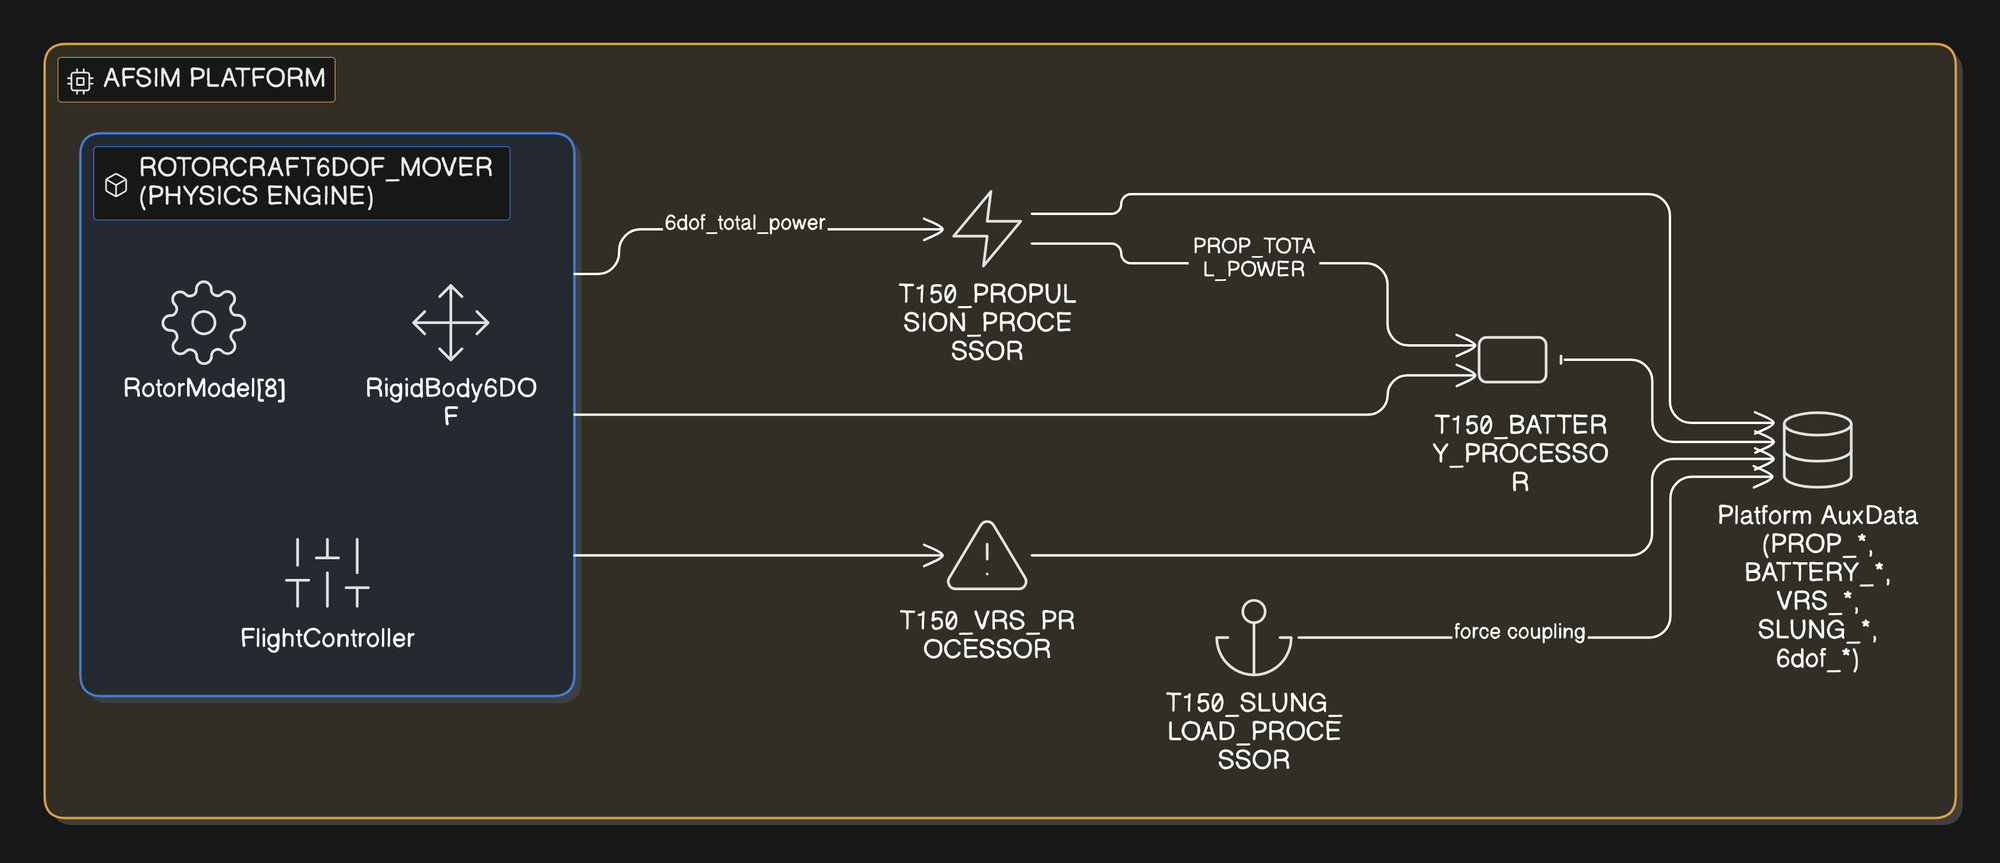
\includegraphics[width=\textwidth,height=0.85\textheight,keepaspectratio]{images/15_UAM_functional_block_diagram.png}
\caption{\unclass T-150 Model Functional Block Diagram}
\label{fig:blockDiagram}
\end{center}
\end{figure}

\unclass \textbf{Data Flow Summary}:
\begin{enumerate}
	\item \unclass The \textbf{6DOF Mover} computes rigid body dynamics and writes total power to AuxData
	\item \unclass The \textbf{Battery Processor} reads power from AuxData (or from the Propulsion Processor) and computes SOC, voltage, current
	\item \unclass The \textbf{Propulsion Processor} models individual motor states, thermal dynamics, and ground effect
	\item \unclass The \textbf{VRS Processor} reads platform velocity from the mover and computes VRS safety margins
	\item \unclass The \textbf{Slung Load Processor} reads platform acceleration and computes pendulum dynamics
	\item \unclass All processors write their state to \textbf{AuxData} for cross-plugin access and scenario script queries
\end{enumerate}

\subsection{\unclass Model Fidelity Log}\label{sec:ModelFidelityLog}

\unclass The model was developed iteratively over six enhancement phases:

\tableFouNow{\unclasslabel}{\unclass Model Fidelity Log}{fidelityLog}
{0.4in}{0.8in}{2in}{3in}{
	Phase & Date & Enhancement & Impact on Fidelity \\
	1 & 2025-11-29 & Thermal parameter fixes, VRS mover integration, motor time constants & Fixed unrealistic thermal behavior; enabled actual VRS detection \\
	2 & 2025-11-29 & Battery voltage sag model (Li-Ion OCV + SOC-dependent resistance) & Added voltage-dependent power delivery modeling \\
	3 & 2025-11-30 & Dynamic power model (battery reads from propulsion) & Battery drain now reflects actual flight conditions \\
	4 & 2025-11-30 & Ground effect (Cheeseman-Bennett) + payload dynamics & Added near-ground thrust augmentation and mass properties \\
	5 & 2025-11-30 & Slung load dynamics (2-DOF spherical pendulum) & Added cable-suspended payload behavior \\
	6 & 2026-01-08 & 6DOF physics mover, velocity-based power model & Full physics-based flight dynamics; power varies with maneuvers \\
}

\subsection{\unclass Key Performance Indicators (KPIs)}\label{sec:KPISummary}

\unclass The following KPIs are the primary metrics used to assess model fidelity and to support analytical conclusions:

\begin{center}
	\begin{longtblr}
		[
		caption={\unclass KPI Summary},
		label={tab:kpiSummary},
		]{
			colspec={|Q[valign=m,l,1.2in]|Q[valign=m,l,1.2in]|Q[valign=m,l,1in]|Q[valign=m,l,1.3in]|Q[valign=m,c,0.8in]|},
			hline{1-Z}={.5pt},
			cell{1}{1}={c=5}{halign=l},
			cell{Z}{1}={c=5}{halign=r},
			row{2}={bg=TableBlue,fg=white,halign=c},
			rowhead=2,
			rowfoot=1,
		}
		\unclasslabel \\
		KPI & Definition & Measured By & Expected Range & Validation \\
		Flight Endurance & Time from takeoff to battery depletion & BATTERY\_SOC reaching 0\% & 14--36 minutes & Partial (14.3 min simulated) \\
		Cruise Range & Distance at cruise speed before battery depletion & Distance integral during cruise & 25--45 km & Partial \\
		Hover Power & Electrical power during stationary hover & PROP\_TOTAL\_POWER in hover & 17--25 kW & Validated (Test 08) \\
		VRS Onset Speed & Descent rate at which VRS begins & VRS\_MARGIN $< 0.8$ & $\sim$4 m/s descent & Validated (VRS suite) \\
		Battery Voltage Sag & Terminal voltage drop under load & BATTERY\_VOLTAGE\_SAG & 0--15 V & Validated (Test 06) \\
		Motor Temperature & Peak motor temperature during operation & PROP\_MAX\_TEMP & 40--120$^\circ$C & Validated (Test 01) \\
		Slung Load Swing & Maximum swing angle of suspended payload & SLUNG\_SWING\_MAG & 0--45$^\circ$ & Validated (slung load suite) \\
		Energy Efficiency & Energy consumed per straight-line km & Wh/km calculation & 315--800 Wh/km & Validated (pattern tests) \\
		\unclasslabel \\
	\end{longtblr}
\end{center}

\pagebreak

%%%%%%%%%%%%%%%%%%%%%%%%%%%%%%%%%%%%%%%%%%%%%%%%%%%%%%%%%%%%%%%%%%%%%%%
%% SECTION 4 -- MODEL COMPONENTS
%%%%%%%%%%%%%%%%%%%%%%%%%%%%%%%%%%%%%%%%%%%%%%%%%%%%%%%%%%%%%%%%%%%%%%%

\section{\unclass Model Components}\label{sec:ModelComponents}

%% -----------------------------------------------------------------
%% 4.1  Rotorcraft 6DOF Mover
%% -----------------------------------------------------------------

\subsection{\unclass Rotorcraft 6DOF Mover}\label{sec:6DOFMover}

\subsubsection{\unclass Component Overview}\label{sec:6DOFOverview}

\unclass The Rotorcraft6DOF\_Mover is a custom AFSIM mover plugin that replaces the built-in \texttt{WSF\_FULL\_ROTORCRAFT\_MOVER} with a full six-degree-of-freedom (6DOF) physics simulation. It provides physics-based flight dynamics using Newton-Euler rigid body equations, momentum theory rotor aerodynamics, and cascaded flight controllers.

\unclass This mover extends the AFSIM \texttt{WsfRouteMover} base class, enabling integration with AFSIM's route/waypoint navigation system while computing motion from first-principles physics rather than parametric tables.

\unclass \textbf{Plugin File}: \texttt{rotorcraft\_6dof.dll} (Windows) / \texttt{librotorcraft\_6dof.so} (Linux)\\
\textbf{AFSIM Type Name}: \texttt{Rotorcraft6DOF\_Mover}\\
\textbf{Lines of Code}: 2,939 across 6 source files

\subsubsection{\unclass Functional Behavior}\label{sec:6DOFFunctionalBehavior}

\unclass The 6DOF mover computes platform motion through the following physics pipeline executed each simulation timestep:

\begin{enumerate}
	\item \unclass \textbf{Navigation}: Read next waypoint from AFSIM route; compute desired position/velocity
	\item \unclass \textbf{Position Controller}: PD controller converts position error to desired velocity
	\item \unclass \textbf{Velocity Controller}: P controller converts velocity error to desired tilt angles
	\item \unclass \textbf{Attitude Controller}: PD controller converts attitude error to desired body moments
	\item \unclass \textbf{Rotor Model}: Compute individual rotor thrust and torque from throttle commands
	\item \unclass \textbf{Force Aggregation}: Sum all forces (gravity, rotor thrust, drag) in NED frame
	\item \unclass \textbf{Rigid Body Integration}: Semi-implicit Euler integration of Newton-Euler equations
	\item \unclass \textbf{State Update}: Update AFSIM platform position, velocity, and attitude
\end{enumerate}

\unclass \textbf{Rigid Body Equations of Motion}:

\unclass Translational dynamics (Newton's second law in NED frame):

\doMyEquation{\unclasslabel}{Translational Dynamics}{translationalDynamics}{
	\mathbf{F}_{net} = m\mathbf{a} = \mathbf{F}_{gravity} + R_{body \to NED} \cdot \mathbf{F}_{thrust} + \mathbf{F}_{drag}
}

\unclass Where:
\begin{itemize}
	\item \unclass $m$ = total mass (kg)
	\item \unclass $\mathbf{a}$ = acceleration in NED frame (m/s$^2$)
	\item \unclass $R_{body \to NED}$ = rotation matrix from body to NED (derived from quaternion)
	\item \unclass $\mathbf{F}_{gravity} = [0, 0, mg]^T$ (NED, down positive)
\end{itemize}

\unclass Rotational dynamics (Euler's equation):

\doMyEquation{\unclasslabel}{Rotational Dynamics}{rotationalDynamics}{
	\mathbf{M} = I\dot{\boldsymbol{\omega}} + \boldsymbol{\omega} \times (I\boldsymbol{\omega})
}

\unclass Where:
\begin{itemize}
	\item \unclass $\mathbf{M}$ = net moment vector (Nm)
	\item \unclass $I$ = inertia tensor (diagonal: $I_{xx}$, $I_{yy}$, $I_{zz}$)
	\item \unclass $\boldsymbol{\omega}$ = angular velocity vector (rad/s)
\end{itemize}

\unclass \textbf{Attitude Representation}: Quaternion-based (avoids gimbal lock):

\doMyEquation{\unclasslabel}{Quaternion Kinematic Equation}{quaternionKinematics}{
	\dot{q} = \frac{1}{2} q \otimes \boldsymbol{\omega}_q
}

\unclass Where $\boldsymbol{\omega}_q = [0, \omega_x, \omega_y, \omega_z]$ is the angular velocity as a pure quaternion.

\unclass \textbf{Integration Method}: Semi-implicit Euler (symplectic):

\doMyEquation{\unclasslabel}{Semi-Implicit Euler Integration}{semiImplicitEuler}{
\begin{aligned}
	\boldsymbol{\omega}(t+\Delta t) &= \boldsymbol{\omega}(t) + \dot{\boldsymbol{\omega}} \cdot \Delta t \\
	q(t+\Delta t) &= q(t) + \dot{q}(t+\Delta t) \cdot \Delta t \\
	\mathbf{v}(t+\Delta t) &= \mathbf{v}(t) + \mathbf{a} \cdot \Delta t \\
	\mathbf{p}(t+\Delta t) &= \mathbf{p}(t) + \mathbf{v}(t+\Delta t) \cdot \Delta t
\end{aligned}
}

\unclass This method preserves energy better than explicit Euler for oscillatory systems.

\unclass \textbf{Rotor Thrust (Momentum Theory)}:

\doMyEquation{\unclasslabel}{Rotor Thrust}{rotorThrust}{
	T = C_T \cdot \rho \cdot n^2 \cdot D^4
}

\unclass Where:
\begin{itemize}
	\item \unclass $C_T$ = thrust coefficient (\thrustCoefficient)
	\item \unclass $\rho$ = air density (1.225 kg/m$^3$ at sea level)
	\item \unclass $n$ = rotational speed (rev/s = RPM/60)
	\item \unclass $D$ = propeller diameter (\propDiameter)
\end{itemize}

\unclass \textbf{Rotor Torque}:

\doMyEquation{\unclasslabel}{Rotor Torque}{rotorTorque}{
	Q = C_Q \cdot \rho \cdot n^2 \cdot D^5
}

\unclass Where $C_Q$ = torque coefficient (\torqueCoefficient).

\subsubsection{\unclass 6DOF Mover Key Performance Indicators}\label{sec:6DOFKPI}

\tableFouNow{\unclasslabel}{\unclass 6DOF Mover KPIs}{moverKPI}
{1.2in}{1.5in}{1.5in}{2in}{
	KPI & Measure & Expected & Validation \\
	Position hold accuracy & Drift during hover (m) & $< 1.0$ m & Test 03: $\sim$1e-17 m/s drift \\
	Attitude recovery & Time to recover from disturbance & $< 5$ s & Test 02: Clean recovery \\
	Velocity tracking & Steady-state error (m/s) & $< 1.0$ m/s & Test 04: 14.49 vs 15.0 m/s \\
	Numerical stability & No NaN/divergence under stress & Bounded & Test 05: Stable under extremes \\
	Max tilt angle & Maximum bank/pitch during maneuvers & 25$^\circ$ & Test 05: 25$^\circ$ achieved \\
}

\subsubsection{\unclass 6DOF Mover Parameters}\label{sec:6DOFParams}

\begin{center}
	\begin{longtblr}
		[
		caption={\unclass 6DOF Mover Parameters},
		label={tab:moverParams},
		]{
			colspec={|Q[valign=m,l,1.2in]|Q[valign=m,c,0.6in]|Q[valign=m,c,0.6in]|Q[valign=m,l,2in]|Q[valign=m,c,0.8in]|},
			hline{1-Z}={.5pt},
			cell{1}{1}={c=5}{halign=l},
			cell{Z}{1}={c=5}{halign=r},
			row{2}={bg=TableBlue,fg=white,halign=c},
			rowhead=2,
			rowfoot=1,
		}
		\unclasslabel \\
		Parameter & Default & Units & Description & User Tunable \\
		\texttt{mass} & 123 & kg & Total platform mass (MTOW) & Yes \\
		\texttt{inertia\_xx} & 2.5 & kg$\cdot$m$^2$ & Roll moment of inertia & Yes \\
		\texttt{inertia\_yy} & 2.5 & kg$\cdot$m$^2$ & Pitch moment of inertia & Yes \\
		\texttt{inertia\_zz} & 4.5 & kg$\cdot$m$^2$ & Yaw moment of inertia & Yes \\
		\texttt{rotor\_diameter} & 0.76 & m & Propeller diameter & Yes \\
		\texttt{arm\_length} & 0.5 & m & Motor arm length from CG & Yes \\
		\texttt{thrust\_coefficient} & 0.10 & -- & $C_T$ for momentum theory & Yes \\
		\texttt{torque\_coefficient} & 0.008 & -- & $C_Q$ for reaction torque & Yes \\
		\texttt{max\_rpm} & 4500 & RPM & Maximum motor RPM & Yes \\
		\texttt{max\_speed} & 30 & m/s & Maximum horizontal speed & Yes \\
		\texttt{max\_climb\_rate} & 8 & m/s & Maximum climb rate & Yes \\
		\texttt{max\_descent\_rate} & 4 & m/s & Maximum descent rate & Yes \\
		\texttt{max\_tilt\_angle} & 25 & deg & Maximum bank/pitch angle & Yes \\
		\texttt{altitude\_kp} & 0.3 & -- & Altitude PID proportional gain & Yes \\
		\texttt{altitude\_ki} & 0.05 & -- & Altitude PID integral gain & Yes \\
		\texttt{altitude\_kd} & 1.2 & -- & Altitude PID derivative gain & Yes \\
		\texttt{position\_kp} & 1.0 & -- & Position PD proportional gain & Yes \\
		\texttt{position\_kd} & 0.1 & -- & Position PD derivative gain & Yes \\
		\texttt{velocity\_kp} & 3.0 & -- & Velocity P gain & Yes \\
		\texttt{attitude\_kp} & 8.0 & -- & Attitude PD proportional gain & Yes \\
		\texttt{attitude\_kd} & 2.0 & -- & Attitude PD derivative gain & Yes \\
		\unclasslabel \\
	\end{longtblr}
\end{center}

\subsubsection{\unclass 6DOF Mover Assumptions, Limitations, and Gaps}\label{sec:6DOFALG}

\unclass \textbf{Assumptions}:
\begin{itemize}
	\item \unclass Rigid body dynamics (no structural flexibility)
	\item \unclass Constant air density (no altitude-dependent atmospheric model)
	\item \unclass Symmetric inertia tensor (diagonal only; no cross-coupling products)
	\item \unclass Instantaneous force application (no actuator dynamics beyond motor time constant)
\end{itemize}

\unclass \textbf{Limitations}:
\begin{itemize}
	\item \unclass Maximum tilt angle capped at 25 degrees (actual aircraft may achieve more aggressive attitudes)
	\item \unclass No wind model --- all flight occurs in still air
	\item \unclass No sensor noise injection (perfect state knowledge for controllers)
	\item \unclass Coaxial rotor interference modeled as a constant factor (0.85), not dynamic
\end{itemize}

\unclass \textbf{Gaps}:
\begin{itemize}
	\item \unclass Inertia values are estimated, not measured from actual T-150 hardware
	\item \unclass No BEMT (Blade Element Momentum Theory) rotor model --- uses simplified momentum theory
	\item \unclass No structural vibration or aeroelastic effects
\end{itemize}

\pagebreak

%% -----------------------------------------------------------------
%% 4.2  Battery Processor
%% -----------------------------------------------------------------

\subsection{\unclass Battery Processor}\label{sec:BatteryProcessor}

\subsubsection{\unclass Component Overview}\label{sec:BatteryOverview}

\unclass The T150\_BATTERY\_PROCESSOR models a 13S Lithium-Ion battery pack with state-of-charge tracking, open-circuit voltage modeling, voltage sag under load, and SOC-dependent internal resistance. It reads dynamic power consumption from the 6DOF mover or Propulsion Processor via AuxData and computes real-time battery state.

\unclass \textbf{Plugin File}: \texttt{t150\_battery.dll} (Windows) / \texttt{libt150\_battery\_processor.so} (Linux)\\
\textbf{AFSIM Type Name}: \texttt{T150\_BATTERY\_PROCESSOR}\\
\textbf{Lines of Code}: 1,139

\subsubsection{\unclass Functional Behavior}\label{sec:BatteryFunctionalBehavior}

\unclass The Battery Processor executes the following computation each update cycle:

\begin{enumerate}
	\item \unclass \textbf{Read Power Demand}: Read \texttt{6dof\_total\_power} or \texttt{PROP\_TOTAL\_POWER} from AuxData (falls back to configured \texttt{hover\_power\_w} if unavailable)
	\item \unclass \textbf{Apply Efficiency}: Divide by motor efficiency to get electrical power
	\item \unclass \textbf{Add Auxiliary Load}: Add avionics/cooling power
	\item \unclass \textbf{Compute OCV}: Calculate open-circuit voltage from SOC using polynomial fit
	\item \unclass \textbf{Compute Internal Resistance}: Apply SOC-dependent resistance multiplier
	\item \unclass \textbf{Solve for Current}: Use quadratic formula to find stable current solution
	\item \unclass \textbf{Compute Terminal Voltage}: OCV minus IR drop
	\item \unclass \textbf{Update Energy Consumed}: Integrate power over timestep
	\item \unclass \textbf{Update SOC}: Calculate remaining state of charge
	\item \unclass \textbf{Check Warnings}: Evaluate low-battery and voltage sag thresholds
	\item \unclass \textbf{Write to AuxData}: Publish all battery state variables
\end{enumerate}

\unclass \textbf{Open-Circuit Voltage (OCV) Model}:

\unclass The OCV follows a polynomial fit to a typical Li-Ion discharge curve:

\doMyEquation{\unclasslabel}{Cell Open-Circuit Voltage}{cellOCV}{
	V_{cell} = a_0 + a_1 \cdot SOC + a_2 \cdot SOC^2 + a_3 \cdot SOC^3
}

\unclass Where:
\begin{itemize}
	\item \unclass $a_0 = 3.0$ V (cutoff voltage per cell)
	\item \unclass $a_1 = 1.2$ (linear term)
	\item \unclass $a_2 = -0.5$ (creates flat middle region)
	\item \unclass $a_3 = 0.5$ (steeper at ends)
\end{itemize}

\unclass Pack voltage:

\doMyEquation{\unclasslabel}{Pack Open-Circuit Voltage}{packOCV}{
	V_{pack} = V_{cell} \times 13
}

\unclass \textbf{Voltage Sag Model}:

\unclass Under load, terminal voltage drops due to internal resistance:

\doMyEquation{\unclasslabel}{Terminal Voltage Under Load}{terminalVoltage}{
	V_{terminal} = V_{OCV} - I \cdot R_{internal}
}

\unclass Since $P = V_{terminal} \cdot I$, combining equations yields a quadratic:

\doMyEquation{\unclasslabel}{Voltage Sag Quadratic Solution}{voltageSagQuadratic}{
	I = \frac{V_{OCV} - \sqrt{V_{OCV}^2 - 4 \cdot R \cdot P}}{2 \cdot R}
}

\unclass The smaller root is selected as the physically meaningful solution (lower current, higher efficiency).

\unclass \textbf{SOC-Dependent Internal Resistance}:

\unclass Internal resistance follows a U-shaped curve:

\doMyEquation{\unclasslabel}{Effective Internal Resistance}{effectiveResistance}{
	R_{eff} = R_{base} \times f(SOC)
}

\unclass Where:
\begin{itemize}
	\item \unclass SOC $> 0.6$: $f = 1.0 + 0.3 \times \frac{(SOC - 0.6)^2}{0.16}$ (peaks $\sim$1.3x at 100\%)
	\item \unclass $0.2 < \text{SOC} < 0.6$: $f = 1.0$ (minimum in middle range)
	\item \unclass SOC $< 0.2$: $f = 1.0 + 2.0 \times \frac{(0.2 - SOC)^2}{0.04}$ (peaks $\sim$3.0x at 0\%)
\end{itemize}

\unclass \textbf{Energy Consumption}:

\doMyEquation{\unclasslabel}{Energy Consumption and SOC Update}{energyConsumption}{
\begin{aligned}
	E_{consumed}(t) &= E_{consumed}(t-1) + P_{total} \cdot \frac{\Delta t}{3600} \\
	SOC &= 1.0 - \frac{E_{consumed}}{E_{capacity}}
\end{aligned}
}

\subsubsection{\unclass Battery Processor Key Performance Indicators}\label{sec:BatteryKPI}

\tableFouNow{\unclasslabel}{\unclass Battery Processor KPIs}{batteryKPI}
{1.2in}{1.5in}{1.5in}{2in}{
	KPI & Measure & Expected & Validation \\
	Energy conservation & SOC tracking error & $< 0.01\%$ & Test 09: $< 0.01\%$ \\
	Voltage sag at full load & Voltage drop (V) & 5--15 V & Test 06: Validated \\
	Low SOC tracking & Correct SOC from non-100\% start & Monotonic decrease & Test 06: Fixed and validated \\
	Flight endurance & Time to battery depletion & 14--36 min & Test 10: 14.3 min \\
	Warning triggers & Low battery / voltage warnings & At configured thresholds & Test 10: All triggered \\
}

\subsubsection{\unclass Battery Processor Parameters}\label{sec:BatteryParams}

\begin{center}
	\begin{longtblr}
		[
		caption={\unclass Battery Processor Parameters},
		label={tab:batteryParams},
		]{
			colspec={|Q[valign=m,l,1.4in]|Q[valign=m,c,0.7in]|Q[valign=m,c,0.5in]|Q[valign=m,l,2in]|Q[valign=m,c,0.7in]|},
			hline{1-Z}={.5pt},
			cell{1}{1}={c=5}{halign=l},
			cell{Z}{1}={c=5}{halign=r},
			row{2}={bg=TableBlue,fg=white,halign=c},
			rowhead=2,
			rowfoot=1,
		}
		\unclasslabel \\
		Parameter & Default & Units & Description & User Tunable \\
		\texttt{battery\_capacity\_wh} & 7000.0 & Wh & Total battery energy capacity & Yes \\
		\texttt{initial\_soc} & 1.0 & 0--1 & Initial state of charge & Yes \\
		\texttt{hover\_power\_w} & 18000.0 & W & Fallback hover power (if dynamic unavailable) & Yes \\
		\texttt{motor\_efficiency} & 0.85 & 0--1 & Motor/ESC electrical efficiency & Yes \\
		\texttt{auxiliary\_power\_w} & 4000.0 & W & Avionics, cooling, other loads & Yes \\
		\texttt{low\_battery\_warning} & 0.20 & 0--1 & SOC threshold for low-battery warning & Yes \\
		\texttt{critical\_battery\_level} & 0.10 & 0--1 & SOC threshold for critical warning & Yes \\
		\texttt{nominal\_voltage} & 46.8 & V & Pack nominal voltage (13S $\times$ 3.6V) & Yes \\
		\texttt{full\_charge\_voltage} & 54.6 & V & Pack full charge voltage (13S $\times$ 4.2V) & Yes \\
		\texttt{cutoff\_voltage} & 39.0 & V & Pack cutoff voltage (13S $\times$ 3.0V) & Yes \\
		\texttt{internal\_resistance} & 0.025 & $\Omega$ & Pack internal resistance & Yes \\
		\texttt{voltage\_sag\_warning} & 42.0 & V & Voltage threshold for sag warning & Yes \\
		\texttt{use\_dynamic\_power} & true & bool & Read power from mover/propulsion AuxData & Yes \\
		\texttt{power\_source\_key} & 6dof\_total\_power & string & AuxData key for dynamic power input & Yes \\
		\texttt{csv\_output\_file} & -- & path & Optional CSV logging file path & Yes \\
		\texttt{update\_interval} & 0.1 & sec & Processor update rate & Yes \\
		\unclasslabel \\
	\end{longtblr}
\end{center}

\subsubsection{\unclass Battery Processor Assumptions, Limitations, and Gaps}\label{sec:BatteryALG}

\unclass \textbf{Assumptions}:
\begin{itemize}
	\item \unclass Li-Ion chemistry with characteristic polynomial discharge curve
	\item \unclass Uniform cell aging across all 13 series cells
	\item \unclass Constant temperature effects on internal resistance (no thermal feedback from environment)
	\item \unclass Motor efficiency is constant across operating range
\end{itemize}

\unclass \textbf{Limitations}:
\begin{itemize}
	\item \unclass No battery degradation over charge/discharge cycles
	\item \unclass No temperature-dependent capacity derating
	\item \unclass Internal resistance model is simplified (no Randles circuit or EIS-based model)
	\item \unclass No cell-level balancing effects modeled
\end{itemize}

\unclass \textbf{Gaps}:
\begin{itemize}
	\item \unclass Actual T-150 battery pack resistance not measured; 25 m$\Omega$ is estimated for pack-level resistance
	\item \unclass OCV polynomial coefficients are generic Li-Ion, not specific to T-150 cell chemistry
	\item \unclass Auxiliary power (4 kW) may be high; typical avionics draw 0.5--2 kW
\end{itemize}

\pagebreak

%% -----------------------------------------------------------------
%% 4.3  Propulsion Processor
%% -----------------------------------------------------------------

\subsection{\unclass Propulsion Processor}\label{sec:PropulsionProcessor}

\subsubsection{\unclass Component Overview}\label{sec:PropulsionOverview}

\unclass The T150\_PROPULSION\_PROCESSOR models the 8-motor coaxial propulsion system including individual motor state tracking (RPM, temperature, efficiency), thrust calculation via momentum theory, motor thermal dynamics, ground effect thrust augmentation, and payload mass management.

\unclass \textbf{Plugin File}: \texttt{t150\_propulsion.dll} (Windows) / \texttt{libt150\_propulsion.so} (Linux)\\
\textbf{AFSIM Type Name}: \texttt{T150\_PROPULSION\_PROCESSOR}\\
\textbf{Lines of Code}: 1,281

\subsubsection{\unclass Functional Behavior}\label{sec:PropulsionFunctionalBehavior}

\unclass The Propulsion Processor computes the following each update cycle:

\begin{enumerate}
	\item \unclass \textbf{Motor RPM}: Calculate target RPM from voltage and KV rating; apply first-order lag
	\item \unclass \textbf{Motor Thrust}: Compute per-motor thrust using momentum theory
	\item \unclass \textbf{Motor Torque}: Compute per-motor reaction torque
	\item \unclass \textbf{Motor Efficiency}: Parabolic model based on RPM ratio
	\item \unclass \textbf{Electrical Power}: Mechanical power divided by efficiency
	\item \unclass \textbf{Thermal Update}: Compute heat generation and dissipation
	\item \unclass \textbf{Ground Effect}: Apply Cheeseman-Bennett thrust augmentation if near ground
	\item \unclass \textbf{Payload}: Track total mass and CG effects
	\item \unclass \textbf{Dynamic Power}: Calculate total power from flight state (velocity, climb, bank)
	\item \unclass \textbf{Write AuxData}: Publish all propulsion state variables
\end{enumerate}

\unclass \textbf{Motor RPM with First-Order Lag}:

\doMyEquation{\unclasslabel}{Motor RPM First-Order Lag}{motorRPMLag}{
\begin{aligned}
	RPM_{target} &= KV \times V_{nominal} \times 0.85 \\
	\alpha &= \frac{\Delta t}{\tau + \Delta t} \\
	RPM_{new} &= RPM_{old} + \alpha \times (RPM_{target} - RPM_{old})
\end{aligned}
}

\unclass Where $\tau = \motorTimeConstant$ (150 ms time constant for U15II with 30'' propeller).

\unclass \textbf{Motor Efficiency (Parabolic Model)}:

\doMyEquation{\unclasslabel}{Motor Efficiency Model}{motorEfficiency}{
\begin{aligned}
	\eta_{RPM} &= 1.0 - 0.5 \times (RPM_{ratio} - 0.7)^2 \\
	\eta_{torque} &= 1.0 - 0.2 \times Torque_{ratio} \\
	\eta &= \eta_{peak} \times \eta_{RPM} \times \eta_{torque}
\end{aligned}
}

\unclass Peak efficiency occurs at approximately 70\% of maximum RPM.

\unclass \textbf{Thermal Model}:

\doMyEquation{\unclasslabel}{Motor Thermal Model}{motorThermalModel}{
\begin{aligned}
	\dot{Q}_{in} &= P_{electrical} \times (1 - \eta) \\
	\dot{Q}_{out} &= k_{cooling} \times (T_{motor} - T_{ambient}) \\
	\frac{dT}{dt} &= \frac{\dot{Q}_{in} - \dot{Q}_{out}}{C_{thermal}}
\end{aligned}
}

\unclass Where:
\begin{itemize}
	\item \unclass $C_{thermal} = \motorThermalMass$ (motor thermal mass)
	\item \unclass $k_{cooling} = \motorCoolingRate$ (forced convection from prop wash)
\end{itemize}

\unclass \textbf{Ground Effect (Cheeseman-Bennett Approximation)}:

\doMyEquation{\unclasslabel}{Ground Effect -- Cheeseman-Bennett}{groundEffect}{
	\frac{T_{IGE}}{T_{OGE}} = \frac{1}{1 - \left(\frac{R}{4h}\right)^2}
}

\unclass Where:
\begin{itemize}
	\item \unclass $R$ = rotor radius (0.38 m)
	\item \unclass $h$ = rotor height above ground
\end{itemize}

\unclass Active below 1 rotor diameter (0.76 m) AGL. Clamped to maximum 30\% thrust boost.

\unclass \textbf{Dynamic Power Model (Phase 6)}:

\doMyEquation{\unclasslabel}{Total Dynamic Power}{totalDynamicPower}{
	P_{total} = P_{induced} + P_{climb} + P_{parasite} + P_{accel}
}

\tableFouNow{\unclasslabel}{\unclass Dynamic Power Components}{dynamicPowerComponents}
{1in}{1.5in}{2in}{1.8in}{
	Component & Symbol & Equation & Notes \\
	Induced Power & $P_{induced}$ & $k \cdot T \cdot v_i$ where $v_i = \sqrt{T/(2\rho A)}$ & Momentum theory \\
	Climb Power & $P_{climb}$ & $m \cdot g \cdot V_{climb}$ & Weight $\times$ vertical speed \\
	Parasite Power & $P_{parasite}$ & $0.5 \cdot \rho \cdot C_d \cdot A_f \cdot V^3$ & Drag at speed \\
	Acceleration Power & $P_{accel}$ & $m \cdot a \cdot V$ & Transient maneuvers \\
}

\unclass Thrust adjustment for bank angle (coordinated turns):

\doMyEquation{\unclasslabel}{Bank Angle Thrust Adjustment}{bankAngleThrust}{
\begin{aligned}
	T_{required} &= \frac{m \cdot g}{\cos(\phi)} \\
	\phi &= \arctan\left(\frac{a_{horizontal}}{g}\right)
\end{aligned}
}

\unclass Where $\phi$ = bank angle estimated from horizontal acceleration.

\subsubsection{\unclass Propulsion Processor Key Performance Indicators}\label{sec:PropulsionKPI}

\tableFouNow{\unclasslabel}{\unclass Propulsion Processor KPIs}{propulsionKPI}
{1.2in}{1.5in}{1.5in}{2in}{
	KPI & Measure & Expected & Validation \\
	Hover power & Electrical power in hover & 17--25 kW & Test 08: 19.5--20.1 kW mechanical \\
	Motor temperature & Equilibrium temperature & 60--90$^\circ$C & Test 01: Stable \\
	Ground effect factor & Thrust multiplier near ground & 1.0--1.3 & Test 07: Functional \\
	Power vs.\ speed & Power variation with airspeed & Cruise $<$ hover & Validated (pattern tests) \\
}

\subsubsection{\unclass Propulsion Processor Parameters}\label{sec:PropulsionParams}

\begin{center}
	\begin{longtblr}
		[
		caption={\unclass Propulsion Processor Parameters},
		label={tab:propulsionParams},
		]{
			colspec={|Q[valign=m,l,1.4in]|Q[valign=m,c,0.7in]|Q[valign=m,c,0.5in]|Q[valign=m,l,2in]|Q[valign=m,c,0.7in]|},
			hline{1-Z}={.5pt},
			cell{1}{1}={c=5}{halign=l},
			cell{Z}{1}={c=5}{halign=r},
			row{2}={bg=TableBlue,fg=white,halign=c},
			rowhead=2,
			rowfoot=1,
		}
		\unclasslabel \\
		Parameter & Default & Units & Description & User Tunable \\
		\texttt{motor\_count} & 8 & -- & Number of motors & Yes \\
		\texttt{kv\_rating} & 100.0 & RPM/V & Motor KV rating & Yes \\
		\texttt{max\_power\_per\_motor} & 3500.0 & W & Maximum power per motor & Yes \\
		\texttt{propeller\_diameter} & 0.76 & m & Propeller diameter (30 in) & Yes \\
		\texttt{coaxial\_efficiency} & 0.85 & 0--1 & Coaxial rotor interference factor & Yes \\
		\texttt{motor\_thermal\_limit} & 120.0 & $^\circ$C & Motor overtemperature threshold & Yes \\
		\texttt{motor\_thermal\_mass} & 1500.0 & J/K & Motor thermal mass & Yes \\
		\texttt{motor\_cooling\_rate} & 20.0 & W/K & Forced convection cooling rate & Yes \\
		\texttt{motor\_time\_constant} & 0.15 & s & RPM response time constant & Yes \\
		\texttt{ground\_effect\_enabled} & true & bool & Enable ground effect modeling & Yes \\
		\texttt{empty\_mass} & 68.0 & kg & Empty aircraft mass & Yes \\
		\texttt{payload\_mass} & 0.0 & kg & Current payload mass & Yes \\
		\texttt{max\_payload\_mass} & 55.0 & kg & Maximum payload capacity & Yes \\
		\texttt{update\_interval} & 0.1 & sec & Processor update rate & Yes \\
		\unclasslabel \\
	\end{longtblr}
\end{center}

\subsubsection{\unclass Propulsion Processor Assumptions, Limitations, and Gaps}\label{sec:PropulsionALG}

\unclass \textbf{Assumptions}:
\begin{itemize}
	\item \unclass All 8 motors operate identically (no individual motor failures modeled)
	\item \unclass Coaxial interference is a constant factor (0.85), not RPM/inflow-dependent
	\item \unclass Air density is constant (sea-level ISA, 1.225 kg/m$^3$)
	\item \unclass Motor efficiency peaks at 70\% RPM (generic assumption for large brushless motors)
\end{itemize}

\unclass \textbf{Limitations}:
\begin{itemize}
	\item \unclass No individual motor failure or degradation modes
	\item \unclass Propeller aerodynamics use simplified momentum theory (no BEMT)
	\item \unclass No blade pitch variation (fixed-pitch propellers)
	\item \unclass Ground effect uses single-rotor approximation (does not model multi-rotor ground effect interaction)
\end{itemize}

\unclass \textbf{Gaps}:
\begin{itemize}
	\item \unclass Motor thermal parameters estimated from motor class, not specific U15II test data
	\item \unclass Coaxial interference factor (0.85) is generic; actual T-150 interference may differ
	\item \unclass No wind/gust model affects propulsion performance
\end{itemize}

\pagebreak

%% -----------------------------------------------------------------
%% 4.4  VRS Processor
%% -----------------------------------------------------------------

\subsection{\unclass VRS Processor}\label{sec:VRSProcessor}

\subsubsection{\unclass Component Overview}\label{sec:VRSOverview}

\unclass The T150\_VRS\_PROCESSOR detects and models Vortex Ring State (VRS) conditions, a dangerous aerodynamic phenomenon where a rotorcraft descends into its own rotor downwash, causing severe loss of lift and control authority. The processor monitors descent rate and forward speed, implements a 5-state machine, and computes lift degradation and control authority factors.

\unclass \textbf{Plugin File}: \texttt{t150\_vrs.dll} (Windows) / \texttt{libt150\_vrs.so} (Linux)\\
\textbf{AFSIM Type Name}: \texttt{T150\_VRS\_PROCESSOR}\\
\textbf{Lines of Code}: 697

\subsubsection{\unclass Functional Behavior}\label{sec:VRSFunctionalBehavior}

\unclass The VRS Processor reads platform velocity from the AFSIM mover each update cycle and evaluates VRS risk:

\begin{enumerate}
	\item \unclass \textbf{Read Velocity}: Get NED velocity from platform mover
	\item \unclass \textbf{Compute Descent Rate}: $V_d = \max(0, V_{down})$ (positive = descending)
	\item \unclass \textbf{Compute Forward Speed}: $V_{fwd} = \sqrt{V_N^2 + V_E^2}$
	\item \unclass \textbf{Compute VRS Margin}: Combined margin from descent rate and forward speed
	\item \unclass \textbf{Update State Machine}: Transition between 5 VRS states
	\item \unclass \textbf{Compute Degradation}: Calculate lift and control authority factors
	\item \unclass \textbf{Write AuxData}: Publish VRS state, margin, and factors
\end{enumerate}

\unclass \textbf{VRS Margin Calculation}:

\unclass Descent margin:

\doMyEquation{\unclasslabel}{VRS Descent Margin}{vrsDescentMargin}{
	m_{descent} = \begin{cases} 1.0 & \text{if } V_d \leq 0 \\ 1.0 - V_d / V_{threshold} & \text{if } 0 < V_d < V_{threshold} \\ -(V_d - V_{threshold}) / V_{threshold} & \text{if } V_d \geq V_{threshold} \end{cases}
}

\unclass Speed margin:

\doMyEquation{\unclasslabel}{VRS Speed Margin}{vrsSpeedMargin}{
	m_{speed} = \min(1.0,\; V_{fwd} / V_{speed\_threshold})
}

\unclass Combined margin:

\doMyEquation{\unclasslabel}{VRS Combined Margin}{vrsCombinedMargin}{
	m = \begin{cases} 1.0 & \text{if } V_{fwd} \geq V_{speed\_threshold} \\ m_{descent} \cdot w + m_{speed} \cdot (1 - w) & \text{otherwise} \end{cases}
}

\unclass Where $w = 1.0 - m_{speed}$ (weighting factor).

\unclass \textbf{State Machine}:

\unclass The VRS processor implements a 5-state machine governing transitions between flight safety states:

\tableThrNow{\unclasslabel}{\unclass VRS State Machine Transitions}{vrsStateTransitions}
{1in}{1.5in}{3in}{
	From State & To State & Condition \\
	CLEAR & CAUTION & margin $< 0.8$ \\
	CAUTION & CLEAR & margin $\geq 1.0$ \\
	CAUTION & ONSET & margin $< 0.5$ \\
	ONSET & RECOVERY & margin $\geq 0.8$ \\
	ONSET & DEVELOPED & margin $< 0.2$ for 2 seconds \\
	DEVELOPED & RECOVERY & margin $\geq 0.5$ \\
	RECOVERY & CLEAR & development cleared \\
}

\unclass \textbf{Performance Degradation Factors}:

\tableThrNow{\unclasslabel}{\unclass VRS Performance Degradation Factors}{vrsDegradation}
{1in}{1.5in}{2in}{
	State & Lift Factor & Control Factor \\
	CLEAR & 1.00 & 1.00 \\
	CAUTION & 0.95 & 1.00 \\
	ONSET & 0.85 & 0.90 \\
	DEVELOPED & 0.40 & 0.50 \\
	RECOVERY & Proportional to development & Proportional \\
}

\subsubsection{\unclass VRS Processor Parameters}\label{sec:VRSParams}

\begin{center}
	\begin{longtblr}
		[
		caption={\unclass VRS Processor Parameters},
		label={tab:vrsParams},
		]{
			colspec={|Q[valign=m,l,1.4in]|Q[valign=m,c,0.7in]|Q[valign=m,c,0.5in]|Q[valign=m,l,2in]|Q[valign=m,c,0.7in]|},
			hline{1-Z}={.5pt},
			cell{1}{1}={c=5}{halign=l},
			cell{Z}{1}={c=5}{halign=r},
			row{2}={bg=TableBlue,fg=white,halign=c},
			rowhead=2,
			rowfoot=1,
		}
		\unclasslabel \\
		Parameter & Default & Units & Description & User Tunable \\
		\texttt{vrs\_descent\_threshold} & 4.0 & m/s & Descent rate for VRS risk & Yes \\
		\texttt{vrs\_speed\_threshold} & 5.0 & m/s & Forward speed for VRS immunity & Yes \\
		\texttt{caution\_margin} & 0.8 & 0--1 & Margin threshold for CAUTION state & Yes \\
		\texttt{induced\_velocity} & 8.5 & m/s & Rotor induced velocity in hover & Yes \\
		\texttt{coaxial\_factor} & 0.85 & 0--1 & Coaxial VRS resistance factor & Yes \\
		\texttt{update\_interval} & 0.05 & sec & High-rate update for VRS detection (20 Hz) & Yes \\
		\unclasslabel \\
	\end{longtblr}
\end{center}

\subsubsection{\unclass VRS Processor Assumptions, Limitations, and Gaps}\label{sec:VRSALG}

\unclass \textbf{Assumptions}:
\begin{itemize}
	\item \unclass VRS boundaries based on momentum theory induced velocity ratio
	\item \unclass Coaxial configuration provides inherent VRS resistance (factor 0.85)
	\item \unclass Recovery requires either forward speed increase or descent rate reduction
\end{itemize}

\unclass \textbf{Limitations}:
\begin{itemize}
	\item \unclass VRS is detected but does not feed back to modify mover dynamics (informational only)
	\item \unclass No turbulence-induced VRS modeling
	\item \unclass Development time (2s to full VRS) is estimated, not measured
\end{itemize}

\unclass \textbf{Gaps}:
\begin{itemize}
	\item \unclass No coaxial-specific VRS boundary data; factor is estimated
	\item \unclass Lift and control degradation factors are representative, not from T-150 flight test
\end{itemize}

\pagebreak

%% -----------------------------------------------------------------
%% 4.5  Slung Load Processor
%% -----------------------------------------------------------------

\subsection{\unclass Slung Load Processor}\label{sec:SlungLoadProcessor}

\subsubsection{\unclass Component Overview}\label{sec:SlungLoadOverview}

\unclass The T150\_SLUNG\_LOAD\_PROCESSOR models cable-suspended payload dynamics using a 2-DOF spherical pendulum model. It computes swing angles, cable tension, and reaction forces on the aircraft from suspended load motion excited by aircraft maneuvers.

\unclass \textbf{Plugin File}: \texttt{t150\_slung\_load.dll} (Windows) / \texttt{libt150\_slung\_load.so} (Linux)\\
\textbf{AFSIM Type Name}: \texttt{T150\_SLUNG\_LOAD\_PROCESSOR}\\
\textbf{Lines of Code}: 825

\subsubsection{\unclass Functional Behavior}\label{sec:SlungLoadFunctionalBehavior}

\unclass The Slung Load Processor integrates pendulum dynamics at 50 Hz:

\begin{enumerate}
	\item \unclass \textbf{Read Aircraft State}: Get velocity and compute acceleration from mover
	\item \unclass \textbf{Compute Excitation}: Aircraft acceleration drives pendulum
	\item \unclass \textbf{Integrate Pendulum Equations}: Semi-implicit Euler at 50 Hz
	\item \unclass \textbf{Compute Cable Tension}: Static + centripetal components
	\item \unclass \textbf{Compute Reaction Forces}: Forces on aircraft from load
	\item \unclass \textbf{Check States}: Detect resonance, overload, or release conditions
	\item \unclass \textbf{Write AuxData}: Publish all slung load state variables
\end{enumerate}

\unclass \textbf{Spherical Pendulum Equations of Motion}:

\doMyEquation{\unclasslabel}{Spherical Pendulum Equations of Motion}{pendulumEOM}{
\begin{aligned}
	\ddot{\theta}_x &= -\frac{g}{L}\sin(\theta_x) - \frac{a_x}{L}\cos(\theta_x) - c \cdot \dot{\theta}_x \\[6pt]
	\ddot{\theta}_y &= -\frac{g}{L}\sin(\theta_y) - \frac{a_y}{L}\cos(\theta_y) - c \cdot \dot{\theta}_y
\end{aligned}
}

\unclass Where:
\begin{itemize}
	\item \unclass $\theta_x$, $\theta_y$ = swing angles in X and Y planes (rad)
	\item \unclass $g = 9.81$ m/s$^2$
	\item \unclass $L$ = cable length (m)
	\item \unclass $a_x$, $a_y$ = aircraft acceleration (excitation source)
	\item \unclass $c$ = cable damping coefficient (1/s)
\end{itemize}

\unclass \textbf{Natural Frequency}:

\doMyEquation{\unclasslabel}{Pendulum Natural Frequency}{pendulumNaturalFreq}{
	f_n = \frac{1}{2\pi}\sqrt{\frac{g}{L}}
}

\unclass For a 5 m cable: $f_n = 0.223$ Hz (4.5 second period).

\unclass \textbf{Cable Tension}:

\doMyEquation{\unclasslabel}{Cable Tension}{cableTension}{
	T = m \cdot (g \cos(\theta) - a_z + L \cdot \omega^2)
}

\unclass Where $\omega = \sqrt{\dot{\theta}_x^2 + \dot{\theta}_y^2}$ (angular velocity magnitude).

\unclass Constraints: $T \geq 0$ (cable cannot push) and $T \leq T_{max}$ (cable strength limit).

\unclass \textbf{Reaction Forces on Aircraft} (body frame):

\doMyEquation{\unclasslabel}{Slung Load Reaction Forces}{slungLoadReactionForces}{
	F_x = T \sin(\theta_x), \quad F_y = T \sin(\theta_y), \quad F_z = T \cos(\theta)
}

\subsubsection{\unclass Slung Load Processor Parameters}\label{sec:SlungLoadParams}

\begin{center}
	\begin{longtblr}
		[
		caption={\unclass Slung Load Processor Parameters},
		label={tab:slungLoadParams},
		]{
			colspec={|Q[valign=m,l,1.4in]|Q[valign=m,c,0.7in]|Q[valign=m,c,0.5in]|Q[valign=m,l,2in]|Q[valign=m,c,0.7in]|},
			hline{1-Z}={.5pt},
			cell{1}{1}={c=5}{halign=l},
			cell{Z}{1}={c=5}{halign=r},
			row{2}={bg=TableBlue,fg=white,halign=c},
			rowhead=2,
			rowfoot=1,
		}
		\unclasslabel \\
		Parameter & Default & Units & Description & User Tunable \\
		\texttt{load\_mass} & 0.0 & kg & Suspended load mass & Yes \\
		\texttt{cable\_length} & 5.0 & m & Cable length & Yes \\
		\texttt{cable\_damping} & 0.1 & 1/s & Air/friction damping coefficient & Yes \\
		\texttt{attach\_point\_z} & 0.5 & m & Attach point below CG & Yes \\
		\texttt{max\_cable\_tension} & 5000.0 & N & Maximum cable tension before failure & Yes \\
		\texttt{resonance\_threshold} & 20.0 & deg & Swing angle for resonance warning & Yes \\
		\texttt{update\_interval} & 0.02 & sec & Dynamics update rate (50 Hz) & Yes \\
		\unclasslabel \\
	\end{longtblr}
\end{center}

\subsubsection{\unclass Slung Load Processor Assumptions, Limitations, and Gaps}\label{sec:SlungLoadALG}

\unclass \textbf{Assumptions}:
\begin{itemize}
	\item \unclass Cable is massless and inextensible
	\item \unclass Load is a point mass (no aerodynamic drag on load)
	\item \unclass Small-angle behavior for linearized natural frequency
	\item \unclass Cable damping is constant (not velocity-dependent)
\end{itemize}

\unclass \textbf{Limitations}:
\begin{itemize}
	\item \unclass 2-DOF spherical pendulum only (no cable elasticity or bending)
	\item \unclass No aerodynamic drag on the suspended load
	\item \unclass No load release/pickup dynamics
	\item \unclass Reaction forces are informational; do not feed back to mover dynamics
\end{itemize}

\unclass \textbf{Gaps}:
\begin{itemize}
	\item \unclass No T-150-specific cable data; damping coefficient is estimated
	\item \unclass Cable breaking strength (5000 N) is generic
	\item \unclass No multi-point suspension modeling
\end{itemize}

\pagebreak

%%%%%%%%%%%%%%%%%%%%%%%%%%%%%%%%%%%%%%%%%%%%%%%%%%%%%%%%%%%%%%%%%%%%%%%
%% SECTION 5 -- MODEL SETUP AND CONFIGURATION
%%%%%%%%%%%%%%%%%%%%%%%%%%%%%%%%%%%%%%%%%%%%%%%%%%%%%%%%%%%%%%%%%%%%%%%

\section{\unclass Model Setup and Configuration}\label{sec:ModelSetup}

\subsection{\unclass Scenario Configuration}\label{sec:ScenarioConfig}

\unclass The T-150 model is configured through AFSIM scenario files (\texttt{.afsim}). There is no GUI; all parameters are set in text-based scenario scripts.

\unclass \textbf{Note}: This section replaces the ODESSA GUI setup section. AFSIM uses text-based scenario configuration rather than a graphical interface.

\subsubsection{\unclass Installation}\label{sec:Installation}

\begin{codebox}
\begin{lstlisting}[language=bash]
# Clone the repository
git clone https://github.com/DSGarrett/project005_t150_uas.git
cd project005_t150_uas

# Build plugins
./ngic_afsim_build.sh

# Install to AFSIM (requires elevated privileges)
sudo ./ngic_afsim_install.sh
\end{lstlisting}
\end{codebox}

\unclass Plugins are installed to:
\begin{itemize}
	\item \unclass Linux: \texttt{/opt/afsim*/lib/wsf\_plugins/} and \texttt{/opt/afsim*/bin/mission\_plugins/}
	\item \unclass Windows: \texttt{C:\textbackslash{}afsim\textbackslash{}AFSIM-2.2505\textbackslash{}lib\textbackslash{}wsf\_plugins\textbackslash{}} and \texttt{C:\textbackslash{}afsim\textbackslash{}AFSIM-2.2505\textbackslash{}bin\textbackslash{}mission\_plugins\textbackslash{}}
\end{itemize}

\subsubsection{\unclass Minimal Platform Definition}\label{sec:MinimalPlatform}

\begin{codebox}
\begin{lstlisting}
platform_type T150_BASIC WSF_PLATFORM
    icon t150

    mover Rotorcraft6DOF_Mover
        mass 123 kg
        max_speed 30 m/s
    end_mover

    processor BATTERY T150_BATTERY_PROCESSOR
        battery_capacity_wh 7000
        use_dynamic_power true
    end_processor

end_platform_type
\end{lstlisting}
\end{codebox}

\subsubsection{\unclass Full Configuration Example}\label{sec:FullConfigExample}

\begin{codebox}
\begin{lstlisting}
platform_type T150_FULL_PHYSICS T150_UAS

    // Battery with voltage sag model
    processor BATTERY_MONITOR T150_BATTERY_PROCESSOR
        battery_capacity_wh    7000.0
        initial_soc            1.0
        nominal_voltage        46.8
        internal_resistance    0.025
        use_dynamic_power      true
    end_processor

    // Propulsion with thermal and ground effect
    processor PROPULSION_MONITOR T150_PROPULSION_PROCESSOR
        motor_count            8
        kv_rating              100
        max_power_per_motor    3500
        propeller_diameter     0.76
        coaxial_efficiency     0.85
        motor_thermal_limit    120
        ground_effect_enabled  true
        empty_mass             68.0
        payload_mass           40.0
    end_processor

    // VRS detection
    processor VRS_MONITOR T150_VRS_PROCESSOR
        vrs_descent_threshold  4.0
        vrs_speed_threshold    5.0
        coaxial_factor         0.85
    end_processor

    // Slung load dynamics
    processor SLUNG_LOAD T150_SLUNG_LOAD_PROCESSOR
        load_mass              25.0
        cable_length           6.0
        cable_damping          0.1
    end_processor

end_platform_type
\end{lstlisting}
\end{codebox}

\subsection{\unclass Model Parameters (Master Table)}\label{sec:MasterParameterTable}

\unclass The following table provides the complete list of all configurable parameters across all plugins:

\begin{center}
	\begin{longtblr}
		[
		caption={\unclass Master Model Parameters},
		label={tab:ParameterTable},
		]{
			colspec={|Q[valign=m,l,1in]|Q[valign=m,l,1.5in]|Q[valign=m,l,1in]|Q[valign=m,c,0.75in]|Q[valign=m,c,0.625in]|Q[valign=m,c,0.7in]|},
			cell{1}{1}={c=6}{halign=l,bg=white,fg=black},
			cell{Z}{1}={c=6}{halign=r,bg=white,fg=black},
			row{2}={bg=TableBlue,fg=white,halign=c},
			hline{3}={.5pt},
			hline{Y}={.5pt},
			rowhead=2,
			rowfoot=1,
		}   \hline
		\unclasslabel \\\hline
		Variable & Description & Default & Component & User Tunable? & Source \\
		\texttt{mass} & Total platform mass & \unclass 123 kg & 6DOF Mover & Yes & [4] \\ \hline
		\texttt{inertia\_xx} & Roll moment of inertia & \unclass 2.5 kg$\cdot$m$^2$ & 6DOF Mover & Yes & Est. \\ \hline
		\texttt{inertia\_yy} & Pitch moment of inertia & \unclass 2.5 kg$\cdot$m$^2$ & 6DOF Mover & Yes & Est. \\ \hline
		\texttt{inertia\_zz} & Yaw moment of inertia & \unclass 4.5 kg$\cdot$m$^2$ & 6DOF Mover & Yes & Est. \\ \hline
		\texttt{rotor\_diameter} & Propeller diameter & \unclass 0.76 m & 6DOF Mover & Yes & [6] \\ \hline
		\texttt{thrust\_coefficient} & $C_T$ for momentum theory & \unclass 0.10 & 6DOF Mover & Yes & [9] \\ \hline
		\texttt{max\_speed} & Max horizontal speed & \unclass 30 m/s & 6DOF Mover & Yes & [11] \\ \hline
		\texttt{battery\_capacity\_wh} & Total battery capacity & \unclass 7000 Wh & Battery & Yes & [5] \\ \hline
		\texttt{nominal\_voltage} & Pack nominal voltage & \unclass 46.8 V & Battery & Yes & [5] \\ \hline
		\texttt{internal\_resistance} & Pack resistance & \unclass 0.025 $\Omega$ & Battery & Yes & Est. \\ \hline
		\texttt{motor\_efficiency} & Motor/ESC efficiency & \unclass 0.85 & Battery & Yes & [6] \\ \hline
		\texttt{motor\_count} & Number of motors & \unclass 8 & Propulsion & No & [4] \\ \hline
		\texttt{kv\_rating} & Motor KV rating & \unclass 100 RPM/V & Propulsion & Yes & [6] \\ \hline
		\texttt{coaxial\_efficiency} & Coaxial interference & \unclass 0.85 & Propulsion & Yes & [9] \\ \hline
		\texttt{motor\_thermal\_mass} & Motor thermal mass & \unclass 1500 J/K & Propulsion & Yes & Est. \\ \hline
		\texttt{motor\_cooling\_rate} & Cooling rate & \unclass 20 W/K & Propulsion & Yes & Est. \\ \hline
		\texttt{vrs\_descent\_threshold} & VRS descent rate & \unclass 4.0 m/s & VRS & Yes & [10] \\ \hline
		\texttt{vrs\_speed\_threshold} & VRS forward speed & \unclass 5.0 m/s & VRS & Yes & [10] \\ \hline
		\texttt{load\_mass} & Slung load mass & \unclass 0.0 kg & Slung Load & Yes & Scenario \\ \hline
		\texttt{cable\_length} & Cable length & \unclass 5.0 m & Slung Load & Yes & Scenario \\ \hline
		\texttt{cable\_damping} & Cable damping & \unclass 0.1 1/s & Slung Load & Yes & Est. \\
		\unclasslabel \\\hline
	\end{longtblr}
\end{center}

\subsection{\unclass Model Specific Log Files}\label{sec:LogFiles}

\unclass The simulation can generate the following output files:

\tableFouNow{\unclasslabel}{\unclass Model Log Files}{logFiles}
{1in}{0.8in}{2.5in}{2in}{
	Output & Format & Content & Configuration \\
	Battery CSV & CSV & SOC, voltage, current, power per timestep & \texttt{csv\_output\_file} parameter \\
	AFSIM AER & AER (binary) & Full simulation event records & \texttt{event\_pipe} in scenario \\
	AFSIM Log & Text & Console output with processor messages & \texttt{log\_file} in scenario \\
	Telemetry CSV & CSV & 6DOF state: position, velocity, attitude & Optional 6DOF logging \\
}

\pagebreak

%%%%%%%%%%%%%%%%%%%%%%%%%%%%%%%%%%%%%%%%%%%%%%%%%%%%%%%%%%%%%%%%%%%%%%%
%% SECTION 6 -- ANALYTIC OUTPUTS
%%%%%%%%%%%%%%%%%%%%%%%%%%%%%%%%%%%%%%%%%%%%%%%%%%%%%%%%%%%%%%%%%%%%%%%

\section{\unclass Analytic Outputs}\label{sec:AnalyticOutputs}

\subsection{\unclass AuxData Output Keys}\label{sec:AuxDataOutputKeys}

\unclass All model state is published to the AFSIM AuxData container, accessible from scenario scripts and other processors. The following tables list all output keys by component.

\unclass \textbf{Battery Processor Outputs}:

\tableFouNow{\unclasslabel}{\unclass Battery Processor AuxData Outputs}{batteryOutputs}
{1.5in}{0.7in}{0.5in}{3.5in}{
	Key & Type & Units & Description \\
	\texttt{BATTERY\_SOC} & double & 0--1 & State of charge \\
	\texttt{BATTERY\_POWER\_W} & double & W & Current power draw \\
	\texttt{BATTERY\_ENERGY\_WH} & double & Wh & Remaining energy \\
	\texttt{BATTERY\_VOLTAGE} & double & V & Terminal voltage under load \\
	\texttt{BATTERY\_OCV} & double & V & Open-circuit voltage \\
	\texttt{BATTERY\_VOLTAGE\_SAG} & double & V & Voltage drop from IR \\
	\texttt{BATTERY\_CURRENT\_A} & double & A & Current draw \\
	\texttt{BATTERY\_LOW} & bool & -- & Low battery warning flag \\
	\texttt{BATTERY\_VOLTAGE\_LOW} & bool & -- & Voltage sag warning flag \\
}

\unclass \textbf{Propulsion Processor Outputs}:

\begin{center}
	\begin{longtblr}
		[
		caption={\unclass Propulsion Processor AuxData Outputs},
		label={tab:propulsionOutputs},
		]{
			colspec={|Q[valign=m,l,1.5in]|Q[valign=m,c,0.7in]|Q[valign=m,c,0.5in]|Q[valign=m,l,3.5in]|},
			hline{1-Z}={.5pt},
			cell{1}{1}={c=4}{halign=l},
			cell{Z}{1}={c=4}{halign=r},
			row{2}={bg=TableBlue,fg=white,halign=c},
			rowhead=2,
			rowfoot=1,
		}
		\unclasslabel \\
		Key & Type & Units & Description \\
		\texttt{PROP\_TOTAL\_THRUST} & double & N & Total thrust output \\
		\texttt{PROP\_TOTAL\_POWER} & double & W & Total electrical power \\
		\texttt{PROP\_SYSTEM\_EFF} & double & 0--1 & System efficiency \\
		\texttt{PROP\_MOTOR\_COUNT} & int & -- & Operational motor count \\
		\texttt{PROP\_MAX\_TEMP} & double & $^\circ$C & Hottest motor temperature \\
		\texttt{PROP\_AVG\_TEMP} & double & $^\circ$C & Average motor temperature \\
		\texttt{PROP\_GROUND\_EFFECT} & double & 1.0--1.3 & Ground effect factor \\
		\texttt{PROP\_ALTITUDE\_AGL} & double & m & Altitude above ground \\
		\texttt{PROP\_TOTAL\_MASS} & double & kg & Aircraft + payload mass \\
		\texttt{PROP\_PAYLOAD\_MASS} & double & kg & Payload mass \\
		\texttt{PROP\_THRUST\_MARGIN} & double & 0--1 & Available thrust reserve \\
		\texttt{PROP\_CG\_OFFSET\_X} & double & m & CG offset X \\
		\texttt{PROP\_CG\_OFFSET\_Y} & double & m & CG offset Y \\
		\texttt{PROP\_CG\_OFFSET\_Z} & double & m & CG offset Z \\
		\texttt{PROP\_OVERLOADED} & bool & -- & Payload exceeds capacity \\
		\texttt{PROP\_FORWARD\_SPEED} & double & m/s & Horizontal speed \\
		\texttt{PROP\_CLIMB\_RATE} & double & m/s & Vertical speed (positive=up) \\
		\texttt{PROP\_BANK\_ANGLE} & double & deg & Estimated bank angle \\
		\texttt{PROP\_ACCEL\_MAG} & double & m/s$^2$ & Horizontal acceleration \\
		\unclasslabel \\
	\end{longtblr}
\end{center}

\unclass \textbf{VRS Processor Outputs}:

\tableFouNow{\unclasslabel}{\unclass VRS Processor AuxData Outputs}{vrsOutputs}
{1.5in}{0.7in}{0.5in}{3.5in}{
	Key & Type & Units & Description \\
	\texttt{VRS\_MARGIN} & double & 0--1 & Safety margin (0=VRS, 1=safe) \\
	\texttt{VRS\_STATE} & int & 0--4 & State (CLEAR=0, CAUTION=1, ONSET=2, DEVELOPED=3, RECOVERY=4) \\
	\texttt{VRS\_LIFT\_FACTOR} & double & 0.4--1.0 & Lift degradation factor \\
	\texttt{VRS\_CONTROL\_FACTOR} & double & 0.5--1.0 & Control authority factor \\
	\texttt{VRS\_DEVELOPMENT} & double & 0--1 & VRS development level \\
	\texttt{VRS\_DESCENT\_RATE} & double & m/s & Current descent rate \\
	\texttt{VRS\_FORWARD\_SPEED} & double & m/s & Current forward speed \\
	\texttt{VRS\_CAUTION} & bool & -- & Caution warning flag \\
	\texttt{VRS\_ONSET} & bool & -- & Onset warning flag \\
	\texttt{VRS\_CRITICAL} & bool & -- & Critical (developed VRS) flag \\
}

\unclass \textbf{Slung Load Processor Outputs}:

\begin{center}
	\begin{longtblr}
		[
		caption={\unclass Slung Load Processor AuxData Outputs},
		label={tab:slungLoadOutputs},
		]{
			colspec={|Q[valign=m,l,1.5in]|Q[valign=m,c,0.7in]|Q[valign=m,c,0.5in]|Q[valign=m,l,3.5in]|},
			hline{1-Z}={.5pt},
			cell{1}{1}={c=4}{halign=l},
			cell{Z}{1}={c=4}{halign=r},
			row{2}={bg=TableBlue,fg=white,halign=c},
			rowhead=2,
			rowfoot=1,
		}
		\unclasslabel \\
		Key & Type & Units & Description \\
		\texttt{SLUNG\_LOAD\_STATE} & int & 0--4 & Load state (DETACHED=0, ATTACHED=1, SWINGING=2, RESONANCE=3, RELEASED=4) \\
		\texttt{SLUNG\_LOAD\_MASS} & double & kg & Load mass \\
		\texttt{SLUNG\_CABLE\_LENGTH} & double & m & Cable length \\
		\texttt{SLUNG\_CABLE\_TENSION} & double & N & Cable tension \\
		\texttt{SLUNG\_SWING\_X} & double & deg & Swing angle X plane \\
		\texttt{SLUNG\_SWING\_Y} & double & deg & Swing angle Y plane \\
		\texttt{SLUNG\_SWING\_MAG} & double & deg & Total swing magnitude \\
		\texttt{SLUNG\_FORCE\_X} & double & N & Reaction force on aircraft X \\
		\texttt{SLUNG\_FORCE\_Y} & double & N & Reaction force on aircraft Y \\
		\texttt{SLUNG\_FORCE\_Z} & double & N & Reaction force on aircraft Z \\
		\texttt{SLUNG\_POS\_X} & double & m & Load position X relative to aircraft \\
		\texttt{SLUNG\_POS\_Y} & double & m & Load position Y \\
		\texttt{SLUNG\_POS\_Z} & double & m & Load position Z \\
		\texttt{SLUNG\_NATURAL\_FREQ} & double & Hz & Natural frequency \\
		\texttt{SLUNG\_RESONANCE} & bool & -- & Resonance warning flag \\
		\unclasslabel \\
	\end{longtblr}
\end{center}

\subsection{\unclass Analytic Use of Outputs}\label{sec:AnalyticUse}

\unclass \textbf{Flight Endurance Analysis}: Monitor \texttt{BATTERY\_SOC} over time to determine total flight time under specific mission profiles. Compare energy consumption rates across different flight patterns.

\unclass \textbf{Vulnerability Assessment}: Monitor \texttt{VRS\_MARGIN} and \texttt{VRS\_STATE} during descent maneuvers to identify vulnerable flight regimes. Low margins indicate flight conditions where the platform is susceptible to loss of control.

\unclass \textbf{Payload Impact Analysis}: Compare \texttt{PROP\_THRUST\_MARGIN} and \texttt{BATTERY\_SOC} depletion rates with and without payload to quantify the operational cost of payload carriage.

\unclass \textbf{Slung Load Stability}: Monitor \texttt{SLUNG\_SWING\_MAG} and \texttt{SLUNG\_CABLE\_TENSION} during maneuvers to identify flight profiles that induce dangerous load oscillations.

\pagebreak

%%%%%%%%%%%%%%%%%%%%%%%%%%%%%%%%%%%%%%%%%%%%%%%%%%%%%%%%%%%%%%%%%%%%%%%
%% SECTION 7 -- SOURCES, ASSUMPTIONS, LIMITATIONS, AND GAPS
%%%%%%%%%%%%%%%%%%%%%%%%%%%%%%%%%%%%%%%%%%%%%%%%%%%%%%%%%%%%%%%%%%%%%%%

\section{\unclass Sources, Assumptions, Limitations, and Gaps}\label{sec:SALG}

\subsection{\unclass Sources}\label{sec:Sources}

\unclass All model parameters are derived from the following open-source references:

\tableThrNow{\unclasslabel}{\unclass Sources}{sources}
{0.3in}{3.5in}{2.5in}{
	\# & Reference & Content Used \\
	{[1]} & DoDI 5000.61, Sep 2024 & VV\&A policy and documentation requirements \\
	{[2]} & MIL-STD-3022, Jan 2008 & VV\&A documentation templates \\
	{[3]} & Army Directive 2024-02 & Software development policy \\
	{[4]} & AAIB South Scarle Accident Report, 2023 & T-150 specifications: MTOW, thrust, configuration \\
	{[5]} & US Patent US20240262499A1, 2024 & Battery topology: 13S, capacity, voltage \\
	{[6]} & T-Motor U15II KV100 Specifications & Motor parameters: KV, max power, dimensions \\
	{[7]} & AFSIM 2.2505 Documentation & Plugin API, mover/processor architecture \\
	{[8]} & Cheeseman \& Bennett, ARC R\&M 3021, 1955 & Ground effect model \\
	{[9]} & Johnson, Helicopter Theory, 1980 & Momentum theory, rotor aerodynamics \\
	{[10]} & Leishman, Principles of Helicopter Aerodynamics, 2006 & VRS theory and boundaries \\
	{[11]} & SURVICE TRV-150 Product Data Sheet, 2024 & Manufacturer specifications \\
}

\subsection{\unclass Overall Assumptions}\label{sec:OverallAssumptions}

\begin{enumerate}
	\item \unclass The T-150 operates in standard atmosphere (ISA) at sea level unless altitude effects are specified
	\item \unclass All 8 motors are identical and operate symmetrically
	\item \unclass The airframe is rigid (no structural deformation under load)
	\item \unclass No wind, turbulence, or atmospheric disturbances are modeled
	\item \unclass Sensor and navigation systems provide perfect state knowledge
	\item \unclass Battery cells are uniform and exhibit identical characteristics
	\item \unclass Payload is rigidly attached (except when using slung load processor)
\end{enumerate}

\subsection{\unclass Overall Limitations}\label{sec:OverallLimitations}

\begin{enumerate}
	\item \unclass \textbf{Flight Endurance Gap}: Simulated endurance (14.3 min) is approximately 40\% of manufacturer specification (36 min). This is attributed to conservative power modeling and high auxiliary power estimates. Analysts should apply appropriate scaling when using endurance results.

	\item \unclass \textbf{No Environmental Effects}: Wind, temperature, humidity, and altitude effects on air density are not modeled. Results represent calm, sea-level conditions.

	\item \unclass \textbf{No Sensor Noise}: All state measurements are perfect. Real-world navigation, attitude estimation, and control will introduce errors not captured in simulation.

	\item \unclass \textbf{Informational VRS}: VRS detection is informational; it does not feed back to modify flight dynamics. In reality, VRS causes significant and potentially unrecoverable loss of lift.

	\item \unclass \textbf{Informational Slung Load Forces}: Slung load reaction forces are computed but do not modify aircraft motion. In reality, a swinging load significantly affects aircraft stability.
\end{enumerate}

\subsection{\unclass Overall Gaps}\label{sec:OverallGaps}

\begin{enumerate}
	\item \unclass \textbf{No flight test data}: No actual T-150 flight test data is available for model validation. All validation is against manufacturer specifications, first-principles physics, and analytical predictions.

	\item \unclass \textbf{Inertia values}: Moments of inertia are estimated from platform geometry and mass distribution, not measured.

	\item \unclass \textbf{Battery chemistry specifics}: OCV curve and internal resistance characteristics use generic Li-Ion parameters, not the specific cell chemistry used in the T-150.

	\item \unclass \textbf{Motor-specific data}: Thermal mass, cooling rate, and efficiency curves are based on the T-Motor U15II class rather than specific test data.
\end{enumerate}

\pagebreak

%%%%%%%%%%%%%%%%%%%%%%%%%%%%%%%%%%%%%%%%%%%%%%%%%%%%%%%%%%%%%%%%%%%%%%%
%% SECTION 8 -- REFERENCES
%%%%%%%%%%%%%%%%%%%%%%%%%%%%%%%%%%%%%%%%%%%%%%%%%%%%%%%%%%%%%%%%%%%%%%%

\section{\unclass References}\label{sec:References}

\begin{enumerate}
	\item \unclass Office of the Under Secretary of Defense for Research and Engineering, ``DoD Instruction 5000.61: DoD Modeling and Simulation Verification, Validation, and Accreditation,'' September 17, 2024.

	\item \unclass Department of Defense, ``MIL-STD-3022: Documentation of Verification, Validation, and Accreditation (VV\&A) for Models and Simulations,'' January 28, 2008.

	\item \unclass Department of the Army, ``Army Directive 2024-02: Software Development,'' 2024.

	\item \unclass Air Accidents Investigation Branch, ``AAIB Investigation to Malloy Aeronautics T-150, South Scarle, Nottinghamshire,'' 2023.

	\item \unclass Malloy Aeronautics, ``Battery Pack Topology for Unmanned Aerial Vehicle,'' US Patent US20240262499A1, 2024.

	\item \unclass T-Motor, ``U15II KV100 Motor Specifications,'' 2024.

	\item \unclass Air Force Research Laboratory, ``AFSIM 2.2505 Documentation: Advanced Framework for Simulation, Integration, and Modeling,'' 2025.

	\item \unclass I.C. Cheeseman and W.E. Bennett, ``The Effect of Ground on a Helicopter Rotor in Forward Flight,'' ARC R\&M 3021, 1955.

	\item \unclass W. Johnson, ``Helicopter Theory,'' Princeton University Press, 1980.

	\item \unclass J.G. Leishman, ``Principles of Helicopter Aerodynamics,'' 2nd ed., Cambridge University Press, 2006.

	\item \unclass SURVICE Engineering / Malloy Aeronautics, ``TRV-150 Heavy-Lift UAS Product Data Sheet,'' 2024.
\end{enumerate}

\pagebreak

%%% - - -   UNCLASSIFIED   - - - %%%
